%SETTINGS{{{
\documentclass[11pt]{iopart}
\usepackage{graphicx}
\usepackage{iopams}

% Fixing iopams poor centering of equations:
\expandafter\let\csname equation*\endcsname\relax
\expandafter\let\csname endequation*\endcsname\relax
\usepackage{amsmath}
%
%}}}
\begin{document}
%TITLE_ABS{{{
\title[]{Magnetic Concentrators for more Efficient Wireless Charging}

\author{Donovan Webb}

\address{Department of Physics,
University of Bath, Bath BA2 7AY, United Kingdom}
\ead{dw711@bath.ac.uk}

\begin{abstract}
A device capable of uniformly concentrating a magnetic field within a
free space cavity will increase the efficiency of magnetic field
sensing and wireless power transmission.
A design for such a magnetic field concentrator, informed by the
transformation optic technique, has previously been shown to
concentrate static fields.
However, for wireless power transmission, an oscillating magnetic
field is required.
Here we explore the efficacy of a magnetic concentrator, comprised of
high permeability MuMetal and high conductivity copper, in oscillating fields with a specific focus on
improving the efficiency of wireless power transmission.
The device is shown to effectively concentrate both static and
oscillating magnetic fields into its interior free space region by a
factor of up to $(3.0\pm0.1)$. An almost $70$ fold increase in the
efficiency of wireless power transfer is shown when using a pair of magnetic
concentrators.
With the development of such devices, the convenience of wireless
power transfer need not come at the cost of low efficiencies.

\end{abstract}
%}}}
%INTRO{{{
\section{Introduction}
%% - Motivation and overview brief description of power transfer problem
The manipulation of magnetic fields is a critical tool for many modern
technologies. Magnetic devices often have efficiencies dependent on
the strength of interaction with an external magnetic field. Examples
include energy harvesting from magnetic fields~\cite{Hirai2000} to
magnetoencephalography brain activity scans by locating small magnetic
gradients~\cite{Cohen1968}. The efficiency of such devices may be increased by
concentrating the desired magnetic field within the area of sensing or
harvesting. 

Magnetic fields may be described by Maxwell's
equations and are guided by materials due to their
optical properties, such as permittivity and permeability. Snell's law
allowed the design of many optical devices
using geometrical lenses~\cite{Pendry2012}, however, with the maturation
of fabrication techniques, many materials may be produced with exotic
anisotropic optical properties~\cite{Smith2004} prompting the development
of transformation optics (TO) --- a modern approach to optical device
design~\cite{Pendry2006}.

Here we describe one such TO designed device; The magnetic
concentrator~\cite{Navau2012}, with a particular focus on its efficacy
in wireless power transmission. We first replicate static field
concentration results~\cite{N2014} and then explore the benefits of
the concentrating shells in both non-resonant and resonant near field
wireless power transmission at various frequencies.

\begin{figure}
  \begin{center}
   \noindent\includegraphics[width=0.65\linewidth]{images/trans_Opt_edit.pdf}
  \end{center}
  \caption{The steps of Transformation Optics. a) A ray (red)
    travelling in untransformed spatial coordinates (black grid)
    follows the path of least time. b) A spatial coordinate
    transformation $A$ is applied to guide the ray along the desired
    path. c) A material (blue) is inserted into the untransformed
    space with corresponding permeabilities and permittivities which mimics
    the spatial coordinate transform $A$ for the ray. }
  \label{fig:TO}
\end{figure}

\subsection{Transformation Optics and Metamaterials}
TO informed the design of many new devices such as perfect
lenses~\cite{Pendry2000}, magnetic-hoses~\cite{Navau2014}, -cloaks~\cite{Sun2017},
-rotators~\cite{Sun2017}, and -concentrators~\cite{Navau2012}. It
can be shown that due to the form invariance of Maxwell's equations, a
spatial coordinate transform is equivalent to the insertion of a
material with specific permeabilities and permittivities. This is shown
conceptually by the three steps of the schematic shown in
figure~\ref{fig:TO}. First, a ray is considered in free Cartesian space
in panel $a$, which due to Fermat's principle of least time will 
follow the horizontal spatial grid lines.  The space is then
transformed arbitrarily in panel $b$ so that the ray adopts the
desired path for the final device. The transformation required, $A$,
to morph the ray now informs the optical properties for the specific
inserted material of panel $c$, which is once again located in
untransformed space.

The form invariance of Faraday's law is
described by the equivalent expressions
\begin{equation}
  \label{ME1}
  \nabla'\times \textbf{E'} = -jw[\mu_0]\textbf{H'}
  ~~~~~~~~\text{and}~~~~~~~~
  \nabla\times \textbf{E} = -jw[\mu']\textbf{H},
\end{equation}
where the first is expressed in transformed coordinate space $x'(x, y,
z), y'(x, y, z), z'(x, y, z)$ and free space permeability $[\mu_0]$,
whilst the second is expressed in untransformed Cartesian space $x, y,
z$ but with some space-dependent permeability $[\mu']$.  Equivalent
expressions exist for the remaining Maxwell equations and similarly
some space-dependant permittivity $[\epsilon']$ is required. The space
dependant permeabilities and permittivities are found by,
\begin{equation}
  \label{eqn:J}
  \mu'=\frac{A\mu_0 A^T}{|A|}
  ~~~~~~~~\text{and}~~~~~~~~
  \epsilon'=\frac{A\epsilon_0 A^T}{|A|},
\end{equation}
where $A$ is the Jacobian matrix describing the transformation of
coordinate systems (e.g. between panel $a$ and panel $b$ in
figure~\ref{fig:TO}). 

The resulting calculated optical properties
may be anisotropic, have arbitrary magnitude and even have
negative refractive index~\cite{Pendry2000}. As bulk materials rarely, if ever, show these
properties, optical metamaterials are often
required~\cite{Smith2004}. 

Metamaterials are often comprised of
repeating units whose dimensions are much smaller than the wavelength
of the interacting radiation. The individual units may
have specific geometry, orientation and optical properties to
selectively interact with incident waves so that the net effect of the
material mimics a bulk substance with different optical properties
than its substituent parts.

\subsection{Magnetic Concentrator}
As described above, a device capable of magnetic field concentration
can increase the efficiency of sensors and energy harvesters.
Utilising TO we may design an optimal field concentrator which fulfils
the following criteria: The magnetic field within a region $A$ is concentrated
into a cavity $B$ where $B$ is free space only. A possible geometry
for this device that has cylindrical symmetry is shown on LHS of
figure~\ref{fig:d_motiv}.  To satisfy these conditions, two coordinate
transforms are applied: First the region $\rho < R_2 - \xi$ is
radially and linearly compressed to the region $\rho < R_1$, where
$\xi$ is a thin `skin' distance; Second, to ensure the continuity of
our transformed space, a high ($k^{th}$) order polynomial radial
expansion of $R_2 - \xi < \rho < R_2$ to the region $R_1 < \rho < R_2$
is made. These transformations are described by the coordinate
transformations,
\begin{equation}
  \label{eqn:transform}
  \begin{split}
\rho' = \frac{R_1}{R_2-\xi}\rho,~~~~~~~~\rho'\in[0,~R_2-\xi)~~\\
\rho' = R_2^{1-k}\rho^k~~~~~~~~~\rho'\in[R_2-\xi,~R_2).
  \end{split}
\end{equation}
By symmetry we see that $\theta$ and $z$ remain unchanged through the
two transformations. The corresponding Jacobians may be found for
these transformations and using (\ref{eqn:J}), the
permeabilities of the required inserted material may be found to be
\begin{equation}
  \label{eqn:mat}
  \begin{split}
 \mu' = \begin{pmatrix}1&0&0\\0&1&0\\0&0&(\frac{R_2-\xi}{R_1})^2\end{pmatrix}~~~~~~~~~~~~~\rho'\in[0,~R_1)~~\\
~~~~~~\mu' = \begin{pmatrix}k&0&0\\0&1/k&0\\0&0&\frac{1}{k}(\frac{\rho'}{R_2})^{2/k-2}\end{pmatrix}~~~~~\rho'\in[R_1,~R_2)
  \end{split}
\end{equation}
Taking the limit $\xi \rightarrow 0$ to concentrate all of
the field within $A$ into $B$, and matching the boundary conditions at
$R_2-\xi$ and at $R_1$, we find that $k \rightarrow \infty$. From this
we find that the required permeability within $B$ is satisfied by free
space whilst a material with radial permeability $\mu_\rho \rightarrow
\infty$ and angular permeability $\mu_\theta \rightarrow 0$ is
required for region $A$. The $z$ components of permeability are ignored
as we assume the cylindrical shell is
infinitely long so the $z$ component must be invariant. A model for
this theoretical shell can be seen guiding an external magnetic field
in the COMSOL simulation (figure~\ref{fig:COMSOL}$a$).

To satisfy these highly anisotropic conditions practically, an
exploration of metamaterials is required. First, the relative magnetic
permeability, $\mu_r$, of a material is defined by
\begin{equation}
  \vec{B} = \mu_0\mu_r \vec{H},
\end{equation}
where $B$ is magnetic induction, $\mu_0$ is vacuum permeability, and
$H$ is the externally applied magnetic field. If $\mu_r$ is large
(paramagnetic material) then the magnetic field density within the
material is larger than the external field resulting in a ``guiding''
of field within the material's interior. If $\mu_r$ is small
(diamagnetic material) then the field density is reduced within the material.
A possible discretized shell construction
is proposed~\cite{N2014} where the high radial permeability is
provided by ferromagnetic materials whilst the angular permeability is
shielded by superconducting material.
MuMetal is a soft ferromagnetic material comprised of annealed
nickel-iron alloy specifically created to possess unusually high
permeability ($\mu_r = 50,000-300,000+$).  The magnetization of
MuMetal responds to externally applied fields by the growth and
shrinkage of individual magnetic domains. By annealing the MuMetal and
removing defects, the individual domains may reshape rapidly in
response to a magnetic field by the unimpeded movement of domain
walls.
By using thin sheets, the
easy axis of magnetization also lies in-plane further enforcing the
field to be guided within the sheets. Superconductors in their
Meissner state ($B = 0$) will exclude all magnetic fields from within
their interior giving a relative permeability of $0$. In an
alternating field, a far cheaper option for blocking the angular
magnetic field component is the use of high conductivity copper
sheeting. From Lenz's law, an oscillating magnetic field perpendicular
to a metal sheet will induce eddy currents which will oppose the
changing field. At an appropriate frequency, which is
proportional to the copper thickness, the effective angular
permeability is reduced to near zero. To approximate the conditions
proposed by TO design, these two materials may be arranged in
alternating angular sheets, as seen in figure~\ref{fig:shells}.

In an external static uniform magnetic
field, the ideal shell will increase the field within region $B$ by a
factor of $R_2/R_1$. Similarly, if a magnetic dipole is surrounded by
the concentrating shell, then the field outside of the shell will be
increased by a factor of $R_2/R_1$. 
%% (Comparison to other conc. techniques:
%% It is known that ferromagnetic materials concentrate magnetic fields
%% within their bulk~\cite{ferro} however, concentration of the field
%% into a free space cavity may be required.)
\begin{figure}
  \begin{center}
    \vspace{-1em}
    \begin{minipage}{0.35\linewidth}
   \noindent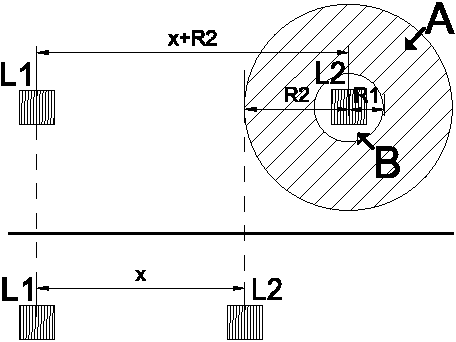
\includegraphics[width=\linewidth]{images/free_space.pdf}
    \end{minipage}
   ~
    \begin{minipage}{0.48\linewidth}
    \vspace{1em}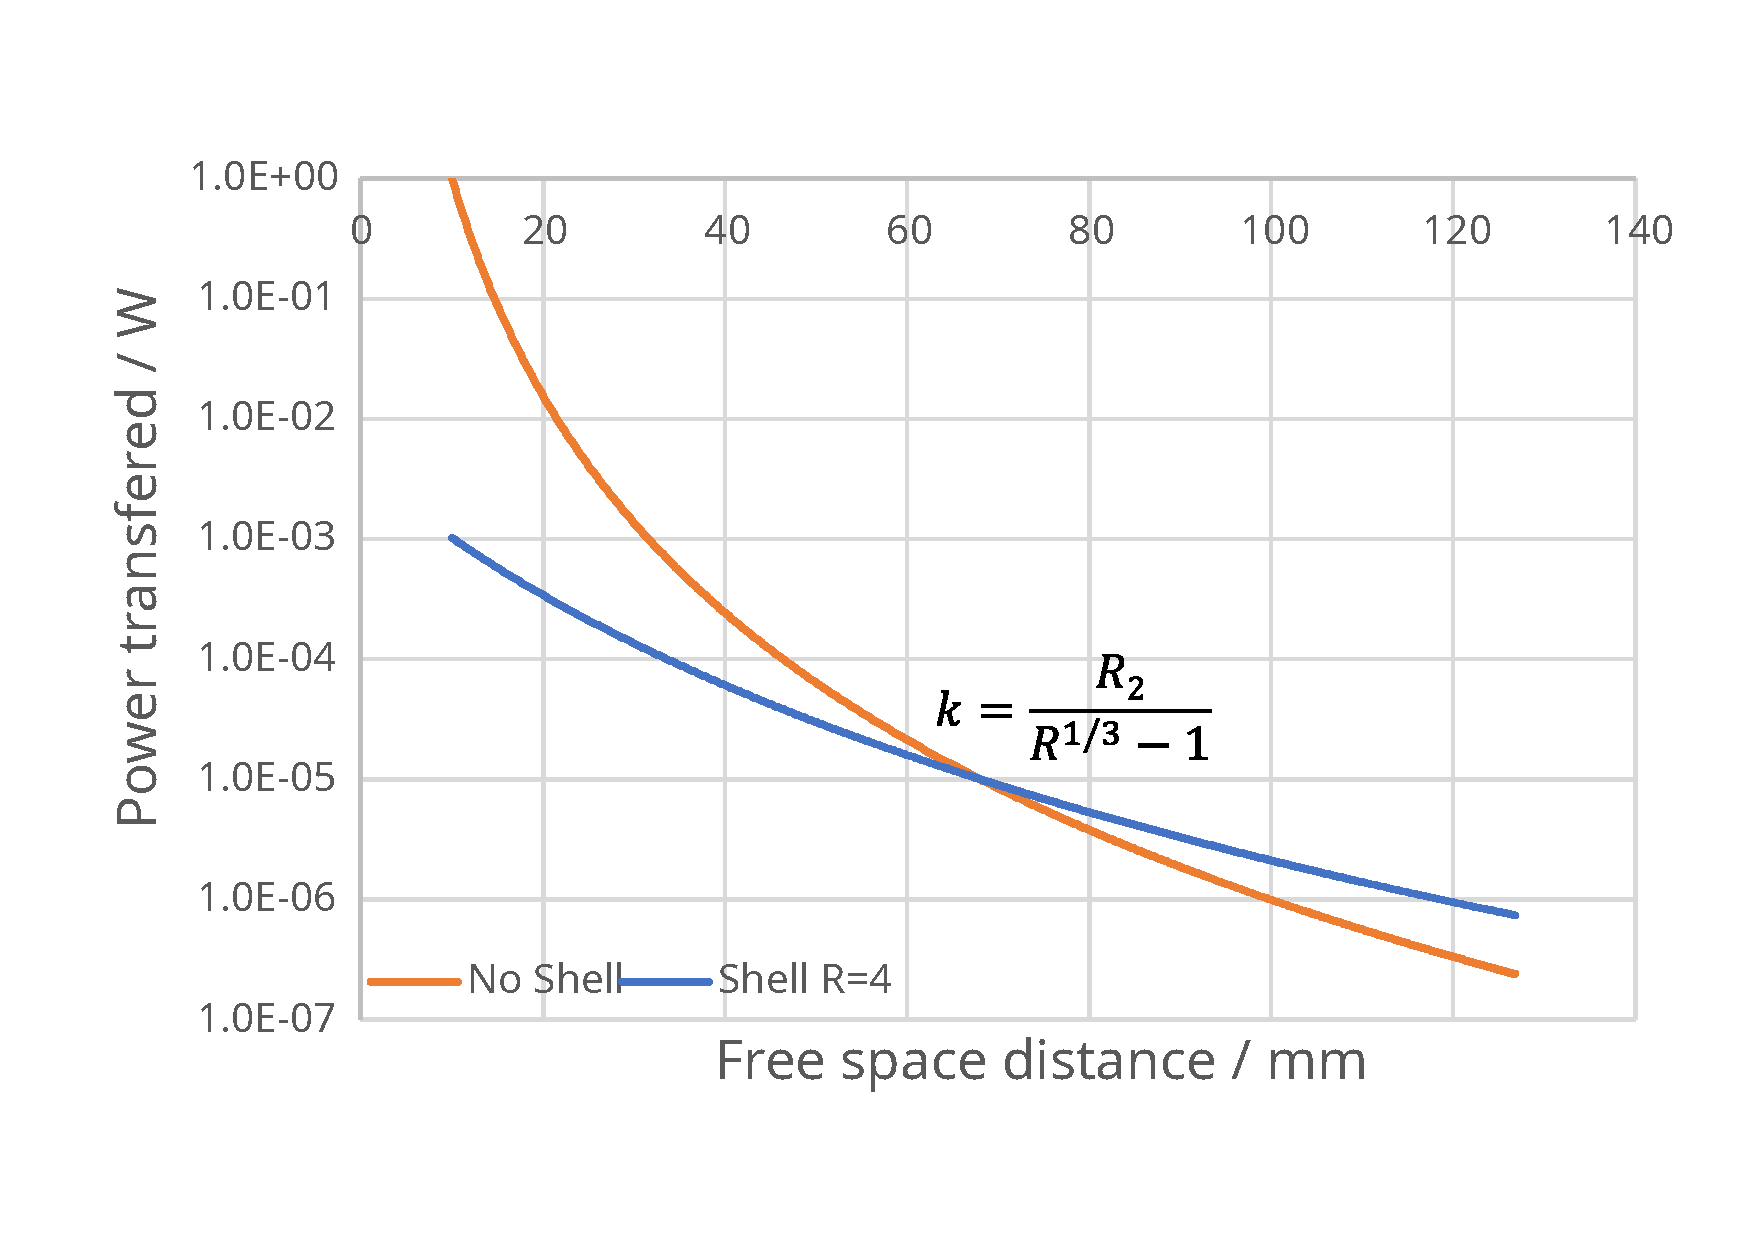
\includegraphics[width=\linewidth]{images/dist_motiv.pdf}
    \end{minipage}
  \end{center}
  \caption{A concentrating shell with inner radius $R_1$ and outer
    radius $R_2$ is useful for increasing the efficiency of wireless
    power transmission by inductive coupling. Power transfer efficiency is highly sensitive
    to the distance between coils being proportional to $r^{-6}$. A
    concentrating shell increases this power transfer by $(R_2/R_1)^2$
    but at the cost of less free space, $x$, between the
    devices. However, at a critical distance $k$, the shell provides
    an improvement over bare dipoles for a given free space distance,
    $x$. LHS: The arrangement of two dipoles (boxes) $L_1$ and $L_2$
    with a fixed free space gap $x$, either with a shell (Top) or
    without (Bottom). RHS: Theoretical power transfer plots for these
    two arrangements when the shell has $R_2 = 40$~mm, $R_1 =
    10$~mm.}\label{fig:d_motiv}
\end{figure}

\begin{figure}
\begin{center}
    \begin{minipage}{0.395\textwidth}
        \noindent\includegraphics[width=\linewidth]{images/shells.png}
    \end{minipage}
    ~~~
    \begin{minipage}{0.423\textwidth}
        \noindent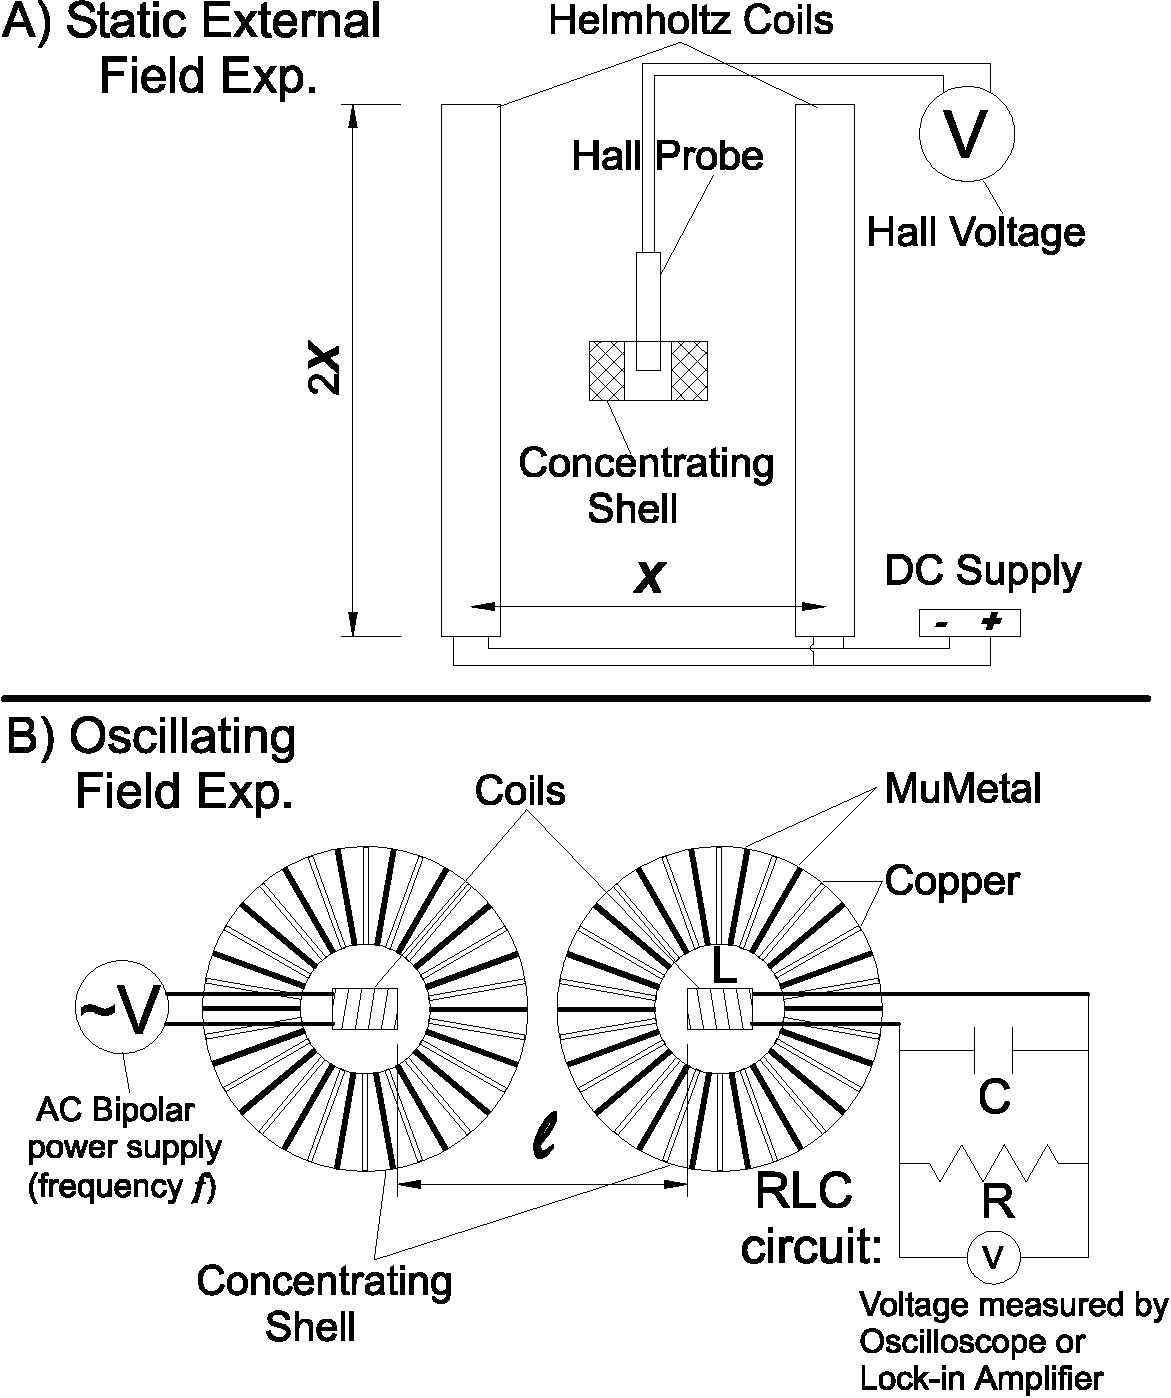
\includegraphics[width=\linewidth]{images/all_schem.pdf}
    \end{minipage}
\caption{LHS: The constructed shells arranged in the power transfer
  experiment. RHS: A) The static field concentration experiment. Using
  a Hall probe to measure magnetic field within the inner radius of
  the shell when an external magnetic field is created by a pair of
  Helmholtz coils. B) The oscillating field concentration experiment
  (power transfer). A coil is driven by an an AC power supply with a
  chosen frequency. A second coil is placed within the field of the
  first so a voltage is induced across it. A resonant RLC circuit is
  constructed incorporating the second coil to maximise power
  transfer.}
\label{fig:shells}
\end{center}
\end{figure}

\begin{figure}
  \begin{center}
   \noindent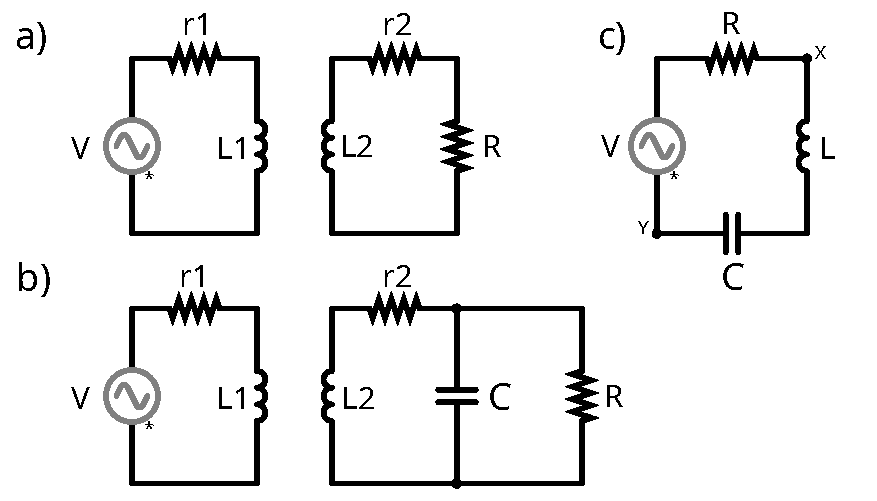
\includegraphics[width=0.65\linewidth]{images/WPT.pdf}
  \end{center}
  \caption{Wireless power transmission by inductive
    coupling. a)~Simple circuitry for coupling $L_1$ and $L_2$
    coils. The useful power transmitted is across load resistance $R$
    whilst power lost is across the internal resistance of coils, $r_1$ and
    $r_2$. b)~The receiving inductor is now part of a resonant RLC
    circuit. c)~A series RLC circuit --- when voltage at $x$ and $y$
    are in phase, the resonant condition is met. d)~An equivalent
    circuit to the coupled inductor circuits but with explicit induced
    voltages shown. }\label{fig:WPT}
\end{figure}


\subsection{Wireless Power Transfer}

The ability to transfer power between devices that are not connected
by wires is useful in many settings: for convenience, e.g. charging mobile
phones; for safety, e.g. implanted medical devices; or for
practicality, e.g. satellites. We shall focus on near field power
transmission by the use of inductive coupling. Inductive coupling
transfers power between two coils of wire (two inductors) by an
oscillating magnetic field.  The transmitting coil is supplied with an
alternating current, which by Ampere's law creates an oscillating
magnetic field. The receiving coil is placed within this magnetic
field so that a current is induced as described by Faraday's law. A
schematic of these two coupled circuits can be seen in
figures~\ref{fig:WPT}$a, b,$ and $d$. This strategy for power transfer
is highly sensitive to distance as the magnetic field of a point dipole
drops off with distance cubed, $r^{-3}$, therefore the power is
proportional to $r^{-6}$ if the dipole is driven at a fixed frequency
and current. If the dipole is a coil of wire with diameter $d$ then
this approximation holds only if $r>>d$.  The power transfer
efficiency, PTE, also suffers with
distance as the non-ideal resistive losses in the primary coil remain
(relatively) constant with distance. To somewhat counteract this sharp
drop off of efficiency with distance, concentrating shells may be used
to magnify the transmitted field and locally concentrate the field
around the receiving coil. The concentrating shell is larger than
the coil by necessity, however, the presence of a shell is always
advantageous when the free space distance between the power
transmitting and power receiving device is greater than $k$~\cite{Prat2016}, where
\begin{equation}
k = \frac{R_2}{\sqrt[3]{R}-1}
\end{equation}
and $R$ is the ratio $R_2/R_1$. This arrangement and the critical
distance $k$ is shown in figure~\ref{fig:d_motiv}.

While the magnetic concentrating shells were designed by TO for static
magnetic fields, in this work we explore their behaviour and efficacy in
oscillating fields of a few kHz, which can be sufficient for practical
power transfer~\cite{Wang2005}.


%% - Wireless power transfer - lit review
%% - Where this work fits in overall field
%%%--------------------------------------------------------------------

%}}}
%METHODS{{{ 
\section{Methods and Circuitry}

\subsection{Construction of shell}
$0.15$~mm MuMetal (MSFHP from Thorlabs) sheets with $\mu_r = 55,000 - 75,000$, and $0.3$~mm high conductivity copper sheets were cut
into $21$~mm by $30$~mm rectangles.  Plastic supports for
holding $36$ sheets of either MuMetal or copper were 3D printed to
produce the shells seen in figure~\ref{fig:shells}. The inner radius
$R_1$ and outer radius $R_2$ were $7$ and $28$~mm respectively to give
an $R_2/R_1$ ratio of 4. The ``Full shell'' contains $36$ sheets of
alternating copper and MuMetal, whilst the ``No shell'' scenario
contains no metal. 

\subsection{DC Magnetic Fields}
Helmholtz coils (RHS figure~\ref{fig:shells}) were powered by constant
DC to create a uniform magnetic field within their
center.
A Hall probe placed at the center of the Helmholtz coils will have a
Hall voltage induced which is proportional to the magnetic field. Once
calibrated the Hall probe can be used to measure the absolute value of
the magnetic field present. A concentrating shell may now be placed at
the center of the Helmholtz coils and the Hall probe placed within the
$R_1$ section of the shells to explore field concentration.
%% described by
%% \begin{equation}
%%   B = \frac{8}{5\sqrt{5}}\frac{\mu_0 nI}{R},
%%   \label{eqn:helm}
%% \end{equation}
%% where $R$ is the radius of the coils, $I$ is the current supplied to
%% the coils, and $n$ is the number of turns of wire.

%%  This equation follows directly from the Biot-Savart law
%% \cite{XXX} and the relative geometry of the coils as seen in
%% figure~\ref{fig:helm}. From equation~\ref{eqn:helm} it can be seen that
%% the magnetic field should increase linearly with supplied
%% current. Using the Hall probe we ensured this was the case and found
%% the relationship of current supplied to magnetic field produced for
%% our paticular Helmholtz arrangement.\\ Now, with the capability to
%% produce known external magnetic fields, the described field
%% concentrating shells may be placed within this field and the Hall
%% probe may be placed within their inner radius to measure concentrated
%% field.

%% \subsection{AC characterization}

%% Use of solenoid, limitations due to pick up.\\
%% Due to the induced voltage across the inductor being small and
%% background noise being high, a lock-in amplifier was used to select
%% only the desired signal frequency. This substantially reduced noise in
%% our readings allowing higher frequency and lower magnetic field
%% strength experiments.\\

\subsection{Power Transfer}
Power transfer experiments measure power dropped across a load
resistor in a receiving circuit versus power lost in the transmitting
circuit's inductor. The receiving circuit, seen in
figure~\ref{fig:WPT}, has multiple arrangements to optimise power
transfer, the simplest of which is the load resistor in series with
the receiving inductor forming an RL circuit with no resonance conditions. Assuming the non-ideal
real resistances of the coil is $r_2 << \omega L$, then the optimal
load resistance for power transfer at some frequency $\omega$ is found
by,
\begin{center}
\begin{minipage}{0.4\linewidth}
\begin{equation}
  V_2 = I_2 (j\omega L_2 + R),  
\end{equation}
\begin{equation}
  P_R = |I_2|^2R = \frac{V_2^2R}{\omega^2L_2^2 + R^2},
  \label{eqn:RL-max-theory}
\end{equation}
\end{minipage}
~~
\vrule
\begin{minipage}{0.4\linewidth}
  $$\text{and setting\quad} \frac{dP_R}{dR} = 0,$$ 
\begin{equation}
  \Rightarrow R = \omega L_2.
  \label{eqn:RL-max}
\end{equation}
\end{minipage}
\end{center}
\vspace{0.2em}
The EMF induced in the receiving coil of a coupled inductance system
may be found by Faraday's law,
\vspace{-0.5em}
\begin{equation}
  \varepsilon = -\frac{d\phi_{21}}{dt},~~~\text{or}~~~\varepsilon = -M\frac{dI_{1}}{dt},
  \label{eqn:M}
\end{equation}
where $\phi_{21}$ is the magnetic flux through coil 2 due to the
current of coil 1 and $M$ is the equivalent mutual inductance between
two coils.
If the current in coil 1 is alternating sinusoidally, then the
maximum EMF induced in coil 2 will be $M I_1 \omega$. Changes in
mutual inductance for different shell constructions is a useful metric
for field concentration as it is proportional to the magnetic flux
present in coil 2. It may also be readily calculated if the current in
coil one is known and the voltage across the load resistance in
circuit 2 is measured at the optimal load resistance
(see (\ref{eqn:RL-max})). This simple relationship of voltage
measurement $V_2$ to mutual inductance $M$ is described by,
\begin{equation}
  V_2 = \frac{MI_1\omega}{\sqrt{2}}.
\label{eqn:MVs}
\end{equation}
It is well known that a resonant RLC arrangement on the receiving
circuit can greatly increase the power transferred in inductive
coupling~\cite{Hirai2000}.  At resonance the complex impedance of the inductance
and capacitance cancel leaving only the load resistance. Our
inductance is assumed to be identical between experiments as the same
coils are used and the capacitance can be found to satisfy the
resonance condition at a chosen operating frequency by the
relationship
\begin{equation}
  C = \frac{1}{\omega^2L}.
  \label{eqn:RLC-res}
\end{equation}
Practically the resonant frequency and required capacitance were found
using a resonant series RLC circuit as seen in
figure~\ref{fig:WPT}$c$ as this method was experimentally
simple and fast. Resonance occurs in this circuit when $V_x$ is in phase with
$V_y$.

The parallel resonant RLC PTE arrangement is considered in
figure~\ref{fig:WPT}$b$ and may be simplified to the equivalent
circuit in $d$, where the voltage across $R_{load}$ is equal to,
\begin{equation}
 V_2 = j\omega MI_1 - j\omega L_2I_2,\quad\text{and}\quad
 I_2 = j\omega MI_1 / Z_2 ,
\end{equation}
where $Z_2$ is the total impedance of circuit 2, which in the case of
a parallel RLC circuit is equivalent to
\begin{equation}
  Z_2 = j\omega L_2 + \frac{1}{j\omega C + R_{load}^{-1}}.
\end{equation}
As with the non-resonant RL case, an optimal resistance must be found to maximise
power transfer. In series RLC the optimal resistance is when
$R_{load}$ matches the sum of internal resistances of the components,
however, in the parallel RLC case, it was found that the optimal
resistance depended non-trivially on the internal resistances of the
components, the frequency, and inductance/capacitance values. The
internal resistances of the inductance was also found to be dependent
on frequency further complicating the optimal resistance calculations.
The optimal resistances were therefore found experimentally through a
resistance sweep at each frequency.  The load voltage can then be
shown to be,
\begin{equation}
    V_2 = A \frac{MR_{opt}}{L_2}I_1,
\label{eqn:RLC-M}
\end{equation}
where $R_{opt}$ is the optimal resistance for power transfer and $A$ is
some constant. Surprisingly there is no explicit dependence of $V_2$ on
frequency, however, it was found that the optimal load resistance had
an implicit dependence on frequency. All the parameters in this
equation may be measured during a PTE experiment allowing the
comparison of relative changes in mutual inductances (and equivalently
magnetic fields) when different concentrating shells are used.

PTE was calculated by finding the power dropped across the load
resistor in circuit 2 and dividing by the power dropped across the
coil in circuit 1. An ideal inductance has voltage and current
$90^\circ$ out of phase meaning the time-averaged power loss is zero,
however real inductors have non-ideal characteristics and so power may
be found by,
\begin{equation}
    P_1 = I_{rms1}V_{rms1}cos(\phi),
\label{eqn:P1}
\end{equation}
where $\phi$ is the phase difference between $I_1$ and $V_1$.

%}}}
%RESULTS{{{
\section{Results}
%DC{{{
\subsection{DC Magnetic Fields}

\begin{figure}
  \begin{center}
   \noindent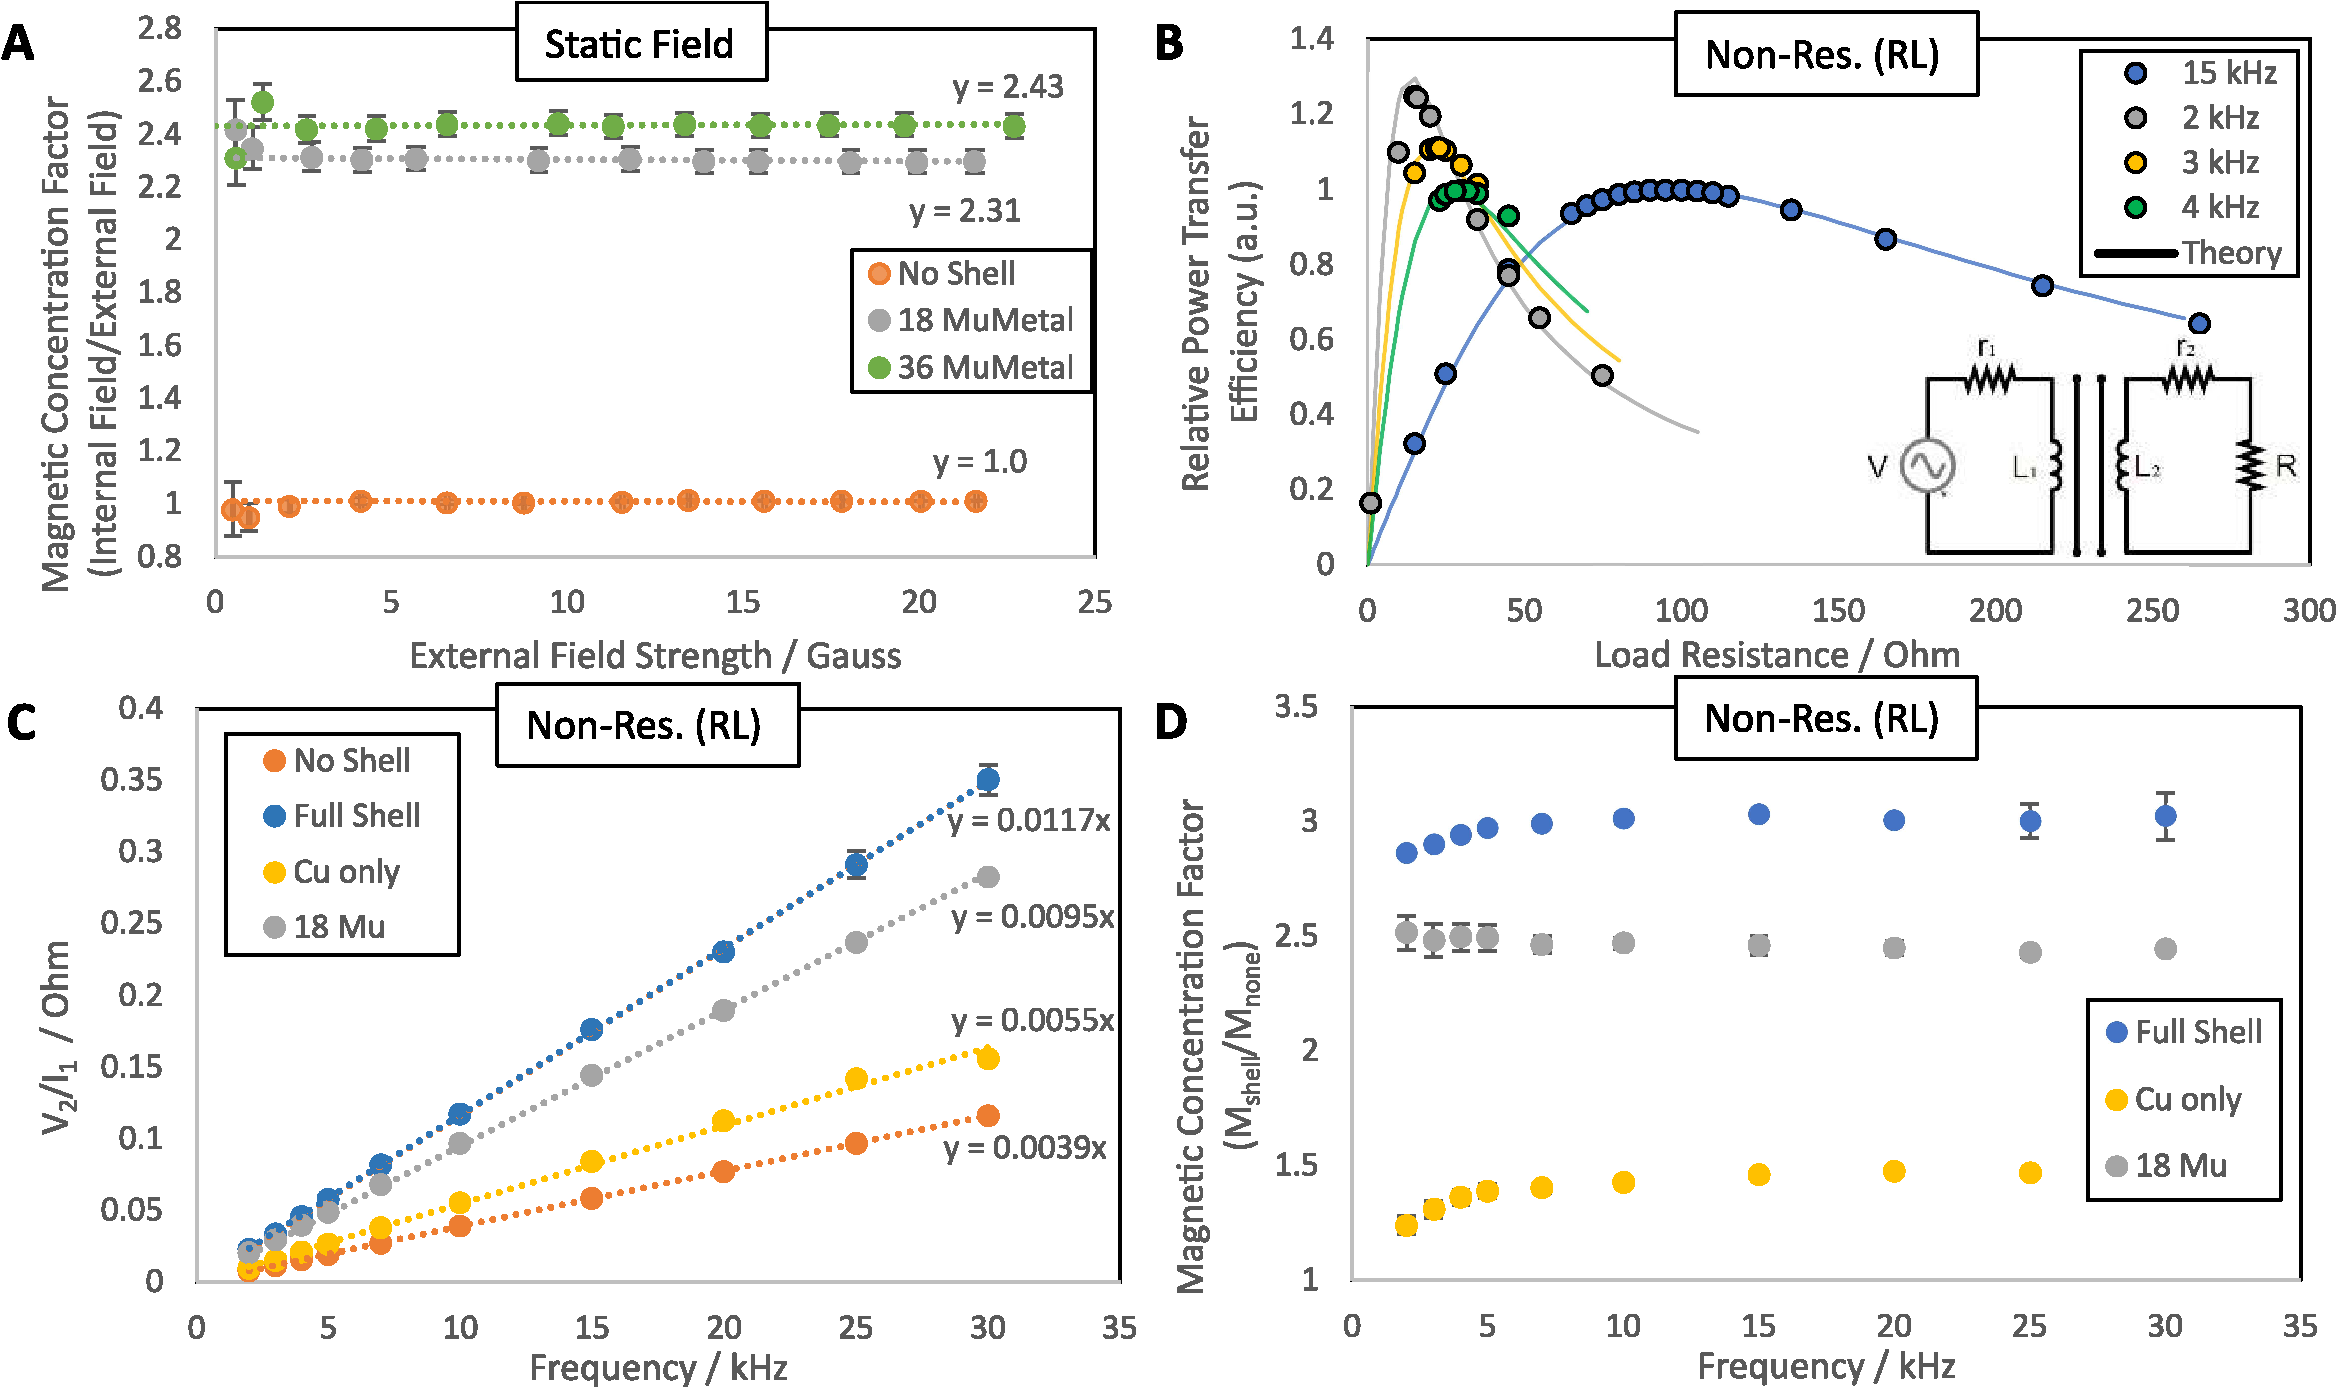
\includegraphics[width=\linewidth]{images/compoundRL-inset.pdf}
  \end{center}
  \caption{
    \textbf{A)} (DC) The concentration of external static fields into
    the interior cavity of shells comprised of either $18$ or $36$
    MuMetal sheets.
    \textbf{B)} (AC) The dependence of relative power transfer
    efficiencies on load resistance in a coupled non-resonant RL
    inductive circuit for various frequencies. Points correspond to
    experimentally measured values whilst the solid lines are found
    using (\ref{eqn:RL-max-theory}).
    \textbf{C)} Finding mutual inductance, $M$, between two coils at a
    fixed distance for various shell configurations in the non-resonant RL circuit
    arrangement.  The gradient is equivalent to $2\pi M/\sqrt{2}$
    from (\ref{eqn:MVs}).
    \textbf{D)} The shell's effect on mutual inductance is found by the
    ratio of ($M$ with shell)/($M$ bare coil). An increase in mutual
    inductance corresponds to an increase in magnetic field density
    within the shell and is shown to be dependant on frequency for
    shells with copper present.}
  \label{fig:DC_RL}
\end{figure}

\begin{figure}
  \begin{center}
   \noindent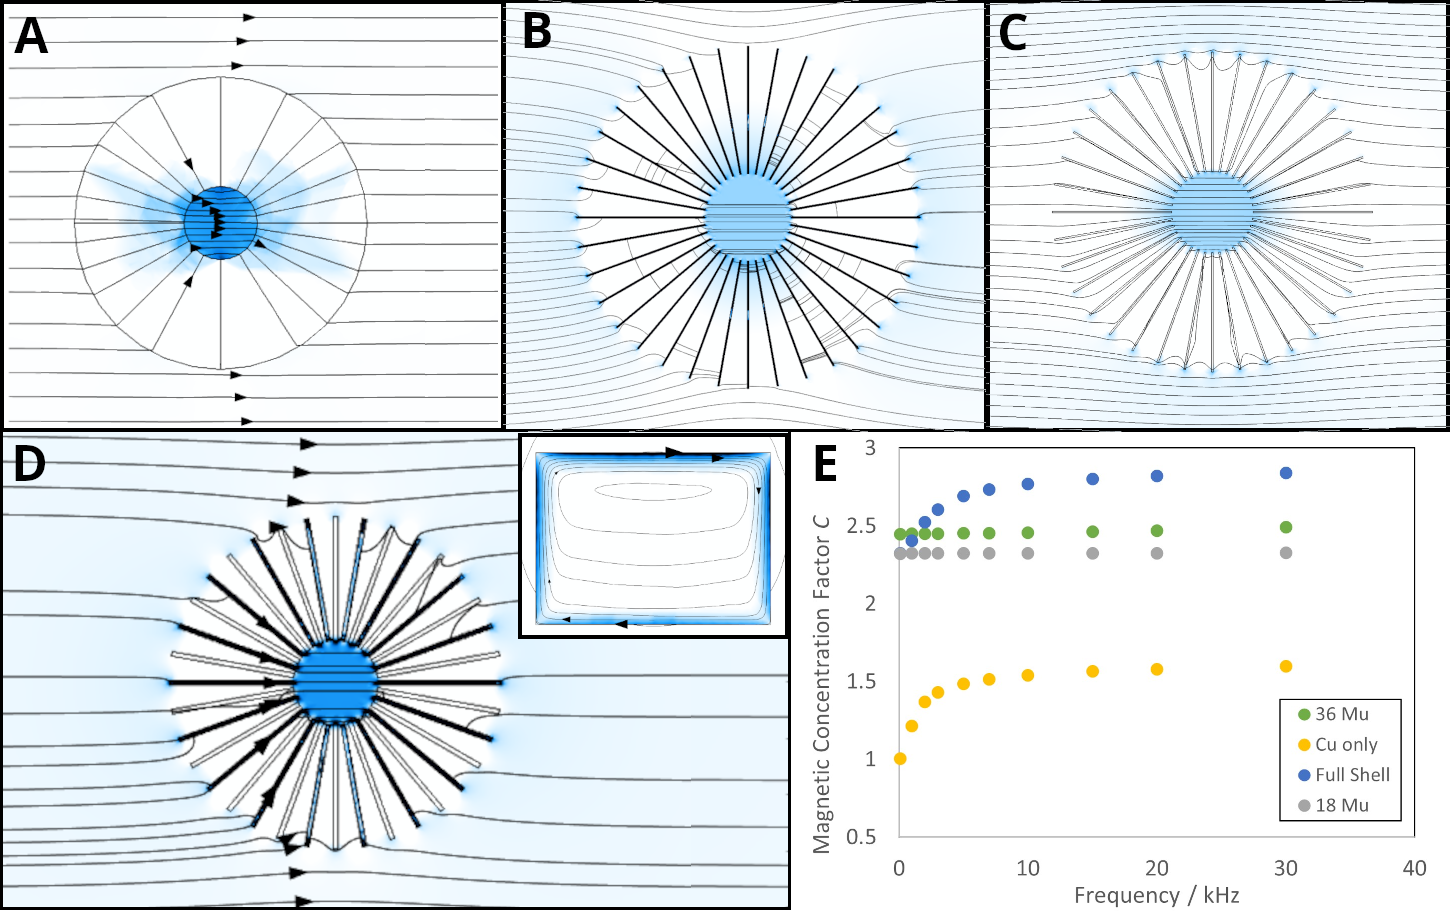
\includegraphics[width=0.89\linewidth]{images/compoundCOMSOL.png}
  \end{center}
  \caption{
    Exploration of magnetic field distributions using the COMSOL
    Multiphysics simulation package.
    \textbf{A)} The perfect anisotropic shell, designed by TO with
    infinite radial permeability and zero angular permeability, in a
    static external magnetic field.
    \textbf{B)} A MuMetal only shell guiding a static field. Note the
    field is guided radially through the interior of the MuMetal but
    angular field is not adequately blocked.
    \textbf{C)} A copper only shell guiding an oscillating external
    magnetic field ($30$~kHz) by effectively shielding the angular component by
    the production of eddy currents.
    \textbf{D)} A full shell comprised of alternating $18$ MuMetal and
    $18$ copper sheets in an oscillating external magnetic field
    ($20$~kHz). The dimensions of the simulated shell match those of
    the real fabricated shells. The MuMetal sheets are darker due to
    guiding the field within their interior whilst the copper sheets
    deflect the angular component of the fields.  The inset image
    displays the eddy current density within a copper sheet when an
    oscillating magnetic field is applied at $45^\circ$.
    \textbf{E)} The dependence of magnetic concentration factor
    ((field within cavity)/(external field)) of various shells on
    frequency of the oscillating field. It can be seen that the two
    shells with copper show improved concentration as frequency is
    increased as predicted and also shown experimentally.
  }
  \label{fig:COMSOL}
\end{figure}

Using Helmholtz coils powered in DC to create a static external
magnetic field (see Methods), we observed constant field concentration
factors within the $R_1$ cavity, across a range of external field
strengths, for various shell constructions. No shell, 18 MuMetal, and
36 MuMetal shells were used and their concentration factor with field
may be seen in figure~\ref{fig:DC_RL}$a$, where concentration factor,
$C$, is defined as (Magnetic field within shell's cavity)/(external
field produced by Helmholtz coils). It was found that the shell
construction of $36$ MuMetal thin sheets gave the optimum
concentration factor of $C_{36} = (2.43\pm0.04)$ with errors likely
due to the sensitivity of dipole orientation within the field. The
$18$ MuMetal shell gave a magnetic concentration factor of $C_{18} =
(2.31\pm0.04)$, which suggests that the shell behaves more ideally
with a greater number of sheets. Simulation work performed on COMSOL
further supports this difference between $18$ and $36$ MuMetal sheets
as shown in figure~\ref{fig:COMSOL}$e$. The absolute values predicted
by COMSOL, $C_{18}= (2.32\pm0.01)$ and $C_{36} = (2.46\pm0.02)$,
closely match the experimentally observed concentration factors for
both cases.
%}}}

\subsection{Power transfer}

\subsection*{Non-resonant power transfer using an RL circuit}
%removed{{{
%% An
%% Oscillating magnetic field, $B$, produced from a solenoid and
%% concentrated by a shell follows,
%% $$B = CI\mu_0n\cos{\omega t},$$ where $C$ is the concentration factor,
%% $I$ is the current through the solenoid and $n$ is the number of turns
%% of the solenoid.  If a second solenoid is placed within the field of
%% the first, as shown in figure~\ref{fig:dipole-dipole}, then voltage
%% will be induced across it according to Faraday's law,
%% $$V = -NA\frac{dB}{dt},$$
%% $$V = C\omega I NA\mu_0n\sin{\omega t},$$
%% where $N$ is the number of turns of the solenoid and $A$ is the area
%% of one turn.
%% The power dropped across a resistor with magnitude $\omega L$ in
%% series with this inductor will then be described by,
%% $$ P = V^2/R $$
%% $$ P = \frac{C^2wI^2k}{L}\sin{\omega t}^2$$
%% where $k$ is the collection of constant coefficients that will remain
%% constant between different shells.  Max power received in the second
%% circuit is therefore proportional to $w \cdot \frac{C^2}{L} \cdot
%% I^2$. Plotting $\frac{P}{I^2}$ against angular frequency $w$ therefore
%% gives $\frac{C^2k}{L}$ as shown in XX figure~\ref{fig:RL-F}. Assuming
%% the coefficients in $k$ remain constant, comparisons of this gradient
%% between a concentrating shell with inductance $L_s$ and no shell with
%% inductance $L_0$ and $C_0 = 1$ yields,
%% \begin{equation}
%%   \eta = \frac{C^2L_0}{L_s},
%%   \label{eqn:eta}
%% \end{equation}
%% the effective concentration factor for power transfer.
%}}}
Power is transferred from the primary circuit to a load resistor in
the secondary circuit in a coupled inductive arrangement as explained
in Methods. This may be simply performed by placing a load resistor in
parallel with the receiving inductor $L_2$ forming an RL circuit with no resonant conditions as
seen in figure~\ref{fig:WPT}$a$. To maximise power transferred, the
optimal load resistance was matched to $R = \omega L$ (see Methods
(\ref{eqn:RL-max})). Figure~\ref{fig:DC_RL}$b$ shows the
relative PTE versus load resistance for various frequencies confirming
the expected optimum load resistance.

Mutual inductances between
the coils (with inductances $L\approx 1$~mH) at a set distance of
$59$~mm were found by: The voltage across the load resistor
in the secondary RL circuit; the current driving the primary
circuit, and using (\ref{eqn:MVs}). The copper only, MuMetal
only, and full copper plus MuMetal shells all showed a concentrating
effect through their relative increases in mutual inductance between the
two coils as shown in figure~\ref{fig:DC_RL}$c$. The full shell
showed an increase of mutual inductance (magnetic field) by a factor
of $(3.0\pm0.1)$, which is nearing the theoretical result from TO of
$R_2/R_1 = 4$ despite only containing $36$ sheets. The frequency
dependence on the relative increase in mutual inductance is shown in
figure~\ref{fig:DC_RL}$d$. The two shell configurations containing
copper are shown to have concentrating effects dependant on
frequency. The concentrating effect rises steeply within the first
$10$~kHz and then plateaus for high frequencies.  This expected
behaviour initially motivated the choice for copper sheets in the
shells for AC power transfer. At higher frequencies the perpendicular
component of alternating magnetic fields produce eddy currents within
the copper which, due to Lenz's law, oppose the change of field
direction and effectively increases the angular permeability of the
shell.  Supporting work done on COMSOL (figure~\ref{fig:COMSOL}$b-e$)
shows a similar observed effect where $36$ copper sheets increases the
concentration factor rapidly from $C = 1$ at $0$~Hz to $C \approx 1.5$
by $10$~kHz and then only a small further increase in efficacy at
higher frequencies.

Apart from errors due to instrument, measurement
reading, and coil placement, we observed noise due to stray magnetic
fields inducing pick-up within cables connecting the coil to the
lock-in amplifier. This source of noise is highly frequency-dependent
and is at the same frequency as our desired signal, so could not be
removed by the use of a lock-in amplifier. To suppress this noise,
cable placement was carefully managed and EM shielding was installed.

\subsection*{Resonant power transfer using an RLC circuit}

\begin{figure}
  \begin{center}
   \noindent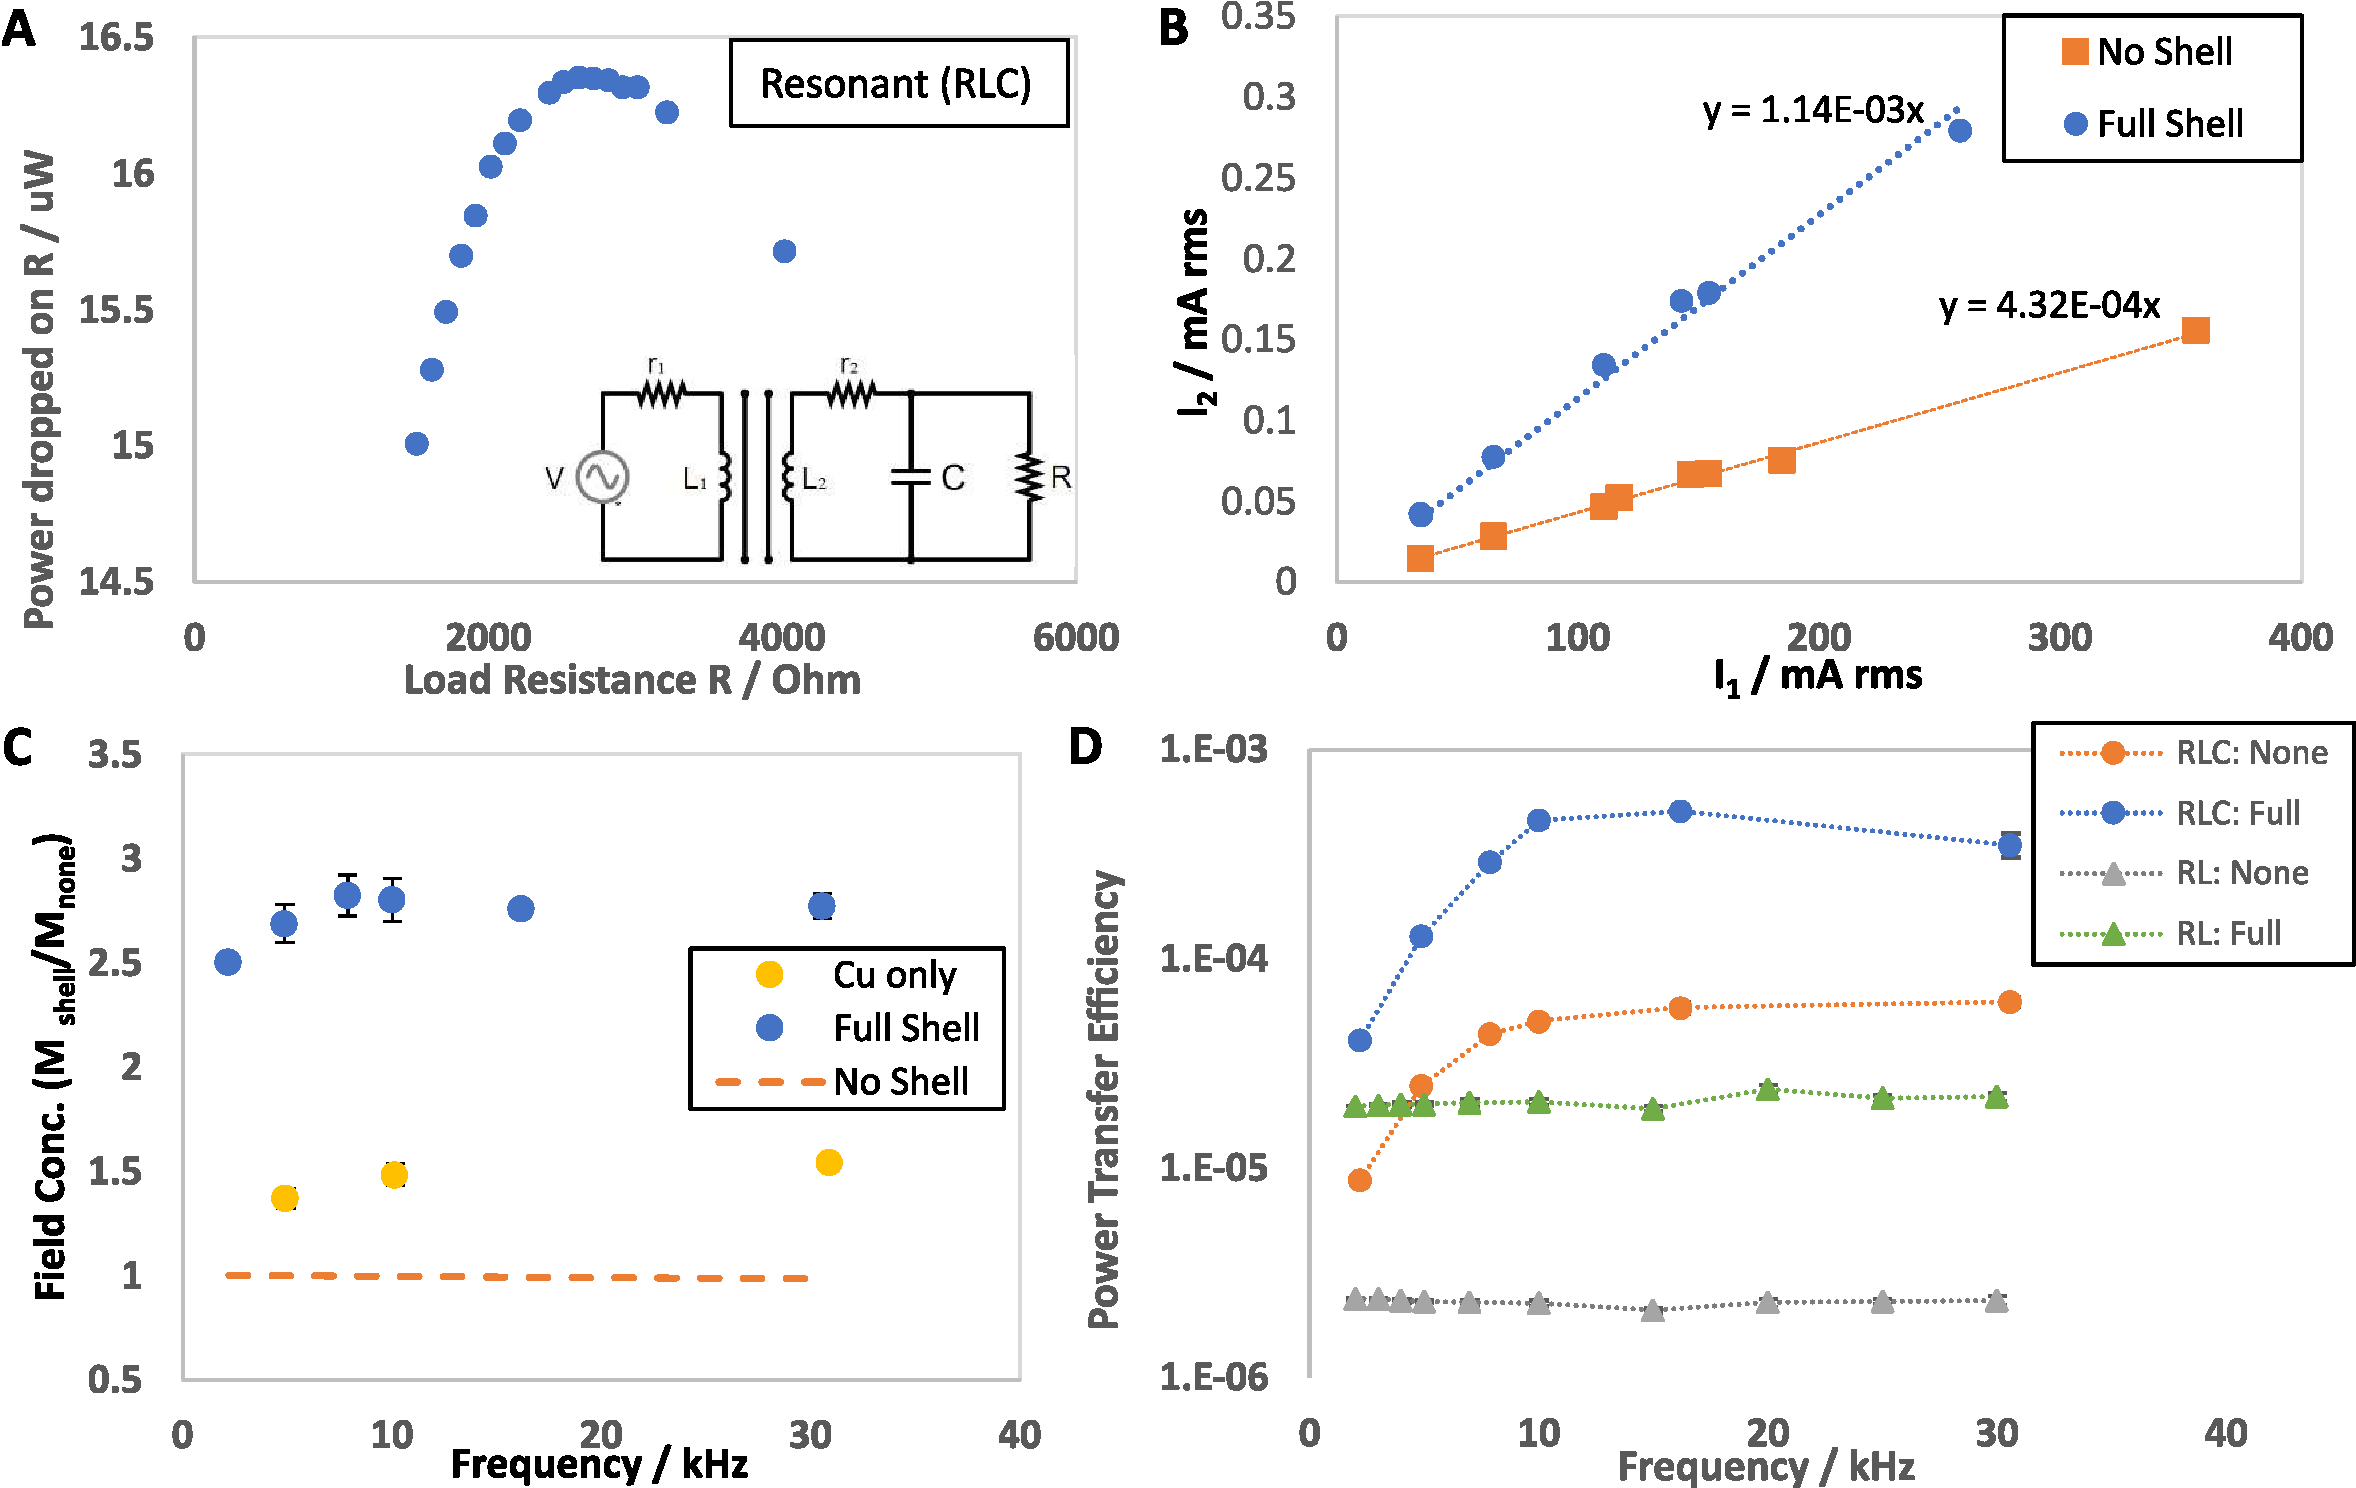
\includegraphics[width=0.9\linewidth]{images/compoundRLC-inset.pdf}
  \end{center}
  \caption{
    \textbf{A)}~Locating the optimal load resistance for power transfer in a resonant
    parallel RLC receiving circuit at an AC frequency of $30$~kHz.
    \textbf{B)}~The current across the optimal load resistance is proportional to
    mutual inductance in the resonant parallel RLC circuit as seen in
    (\ref{eqn:RLC-M}). Voltage across the transmitting coil
    remained constant and so various $I_1$ were achieved by using
    different resonant frequencies. Comparing the gradients of $I_2$
    against $I_1$ for the case when a shell is present to when one is
    not gives the factor increase of mutual inductance which
    is equivalent to the concentration of the field within the shell.
    \textbf{C)}~The shell's effect on mutual inductance in an RLC circuit is
    found by the ratio of ($M$ with shell)/($M$ bare coil). As with
    the RL circuit, the concentration of field is dependant on
    frequency for the full shell which has copper present.
    \textbf{D)}~A comparison of power transfer efficiencies (PTE) for both a
    full shell (18 copper and 18 MuMetal sheets) and no shell in either
    the non-resonant RL or resonant RLC case. PTE is given as a ratio of power dropped
    across the load resistor against power lost in the transmitting
    coil as explained in Methods.
  }
  \label{fig:cpdRLC}
\end{figure}

Resonant parallel RLC circuits are more fitting for optimising power
transfer (see Methods). For the arrangement
described in figure~\ref{fig:WPT}$b$, a full shell comprised of $18$
MuMetal and $18$ copper sheets was explored. The optimal load
resistances were found experimentally by measuring power for a sweep
of resistances, an example of which is shown in
figure~\ref{fig:cpdRLC}$a$ for a field frequency of $30$~kHz.

From (\ref{eqn:RLC-M}), the voltage measured across the load
resistor is proportional to the mutual inductance between the two
coils when the optimal load resistor is used, and the resonance
condition for the RLC circuit is met. Figure~\ref{fig:cpdRLC}$b$
confirms this relationship and shows an increase in mutual inductance
when the full concentrating shell is present. The gradient was found
to be increased by a factor of $(2.6 \pm 0.2)$ corresponding to a field
concentration of the same factor if the inductance of $L_2$ is assumed
to remain constant (see Discussion). 

The dependence of frequency on concentration factor is shown in
figure~\ref{fig:cpdRLC}$c$ and it can be seen that, as with the non-resonant RL and
simulated experiments, the presence of copper in the shell leads to a
low initial concentration which increases with frequency until around
$10$~kHz at which point the concentration factor plateaus.

The PTE for non-resonant RL and resonant RLC, no shell and full shell arrangements are
compared in figure~\ref{fig:cpdRLC}$d$. It can be seen that the shell
increases the efficiency in both cases by a similar factor and that
the parallel resonant RLC arrangement gives a much greater efficiency
than using the simpler RL circuitry. The optimal power transfer
efficiency achieved at $30$~kHz and $59$~mm with one ``full'' shell was
$(0.035\pm0.005)\%$. 

A second ``full'' shell with the same dimensions was placed around the
transmitting coil (seen in figure~\ref{fig:shells}) and this further
increased PTE to $(0.35\pm0.02)\%$. This second shell gave a power
increase of around a factor of $10$ which corresponds to a further
field concentration of $\sqrt{10} \approx 3.2$. To explore the
efficacy of this approach at closer distances the two coils were
separated by $49$~mm yielding a PTE of $(0.015\pm0.004)\%$ with no
shells and $(1.0\pm0.1)\%$ with two full shells. The use of two
concentrating shells displayed an almost $70$ fold increase in
efficiency.
%distance{{{
%% To further explore PTE, the distance between the two coils was
%% varied. With a distance of XXX mm and a full shell around the
%% receiving coil, a PTE of XXX\% was achieved.\\
%% It was expected that a shell around the transmitting coil would
%% further increase the field incident on the receiving coil. Therefore
%% the arrangement described in Methods Figure~\ref{fig:two_shell} was
%% constructed and the peak power transfer observed at $30510$ kHz was
%% found to be $1.01\%$.\\


%% % INCLUDE? A summary of PTE and field concentration factors is shown in the table~\fig{table:summary}.\\

%% \subsection{Distance}
%% Experimentally we found that power drops off as $r^{-5.6}$ which is in
%% close agreement to the theoretical $r^{-6}$.\\
%}}}
%}}}
%DISCUSSION{{{
\section{Discussion}
%% - Tee and Pi circuit analysis
%% - Models
%% - Overall trends matching simulation, analysis and Experimental
%% - Comparison with other published results
%% - Contextualize findings in light of other work

% Non ideal behaviour \\
For the constructed shells used in these experiments, their $R_2/R_1$
ratio was $(4.0\pm0.2)$ and from the theoretical TO work, it was
predicted that the field should be concentrated in the perfect shell
by the same ratio. The greatest concentration of field we observed was
$C_{full} = (3.0\pm0.1)$ in the AC non-resonant RL case. This concentration is
still well below the expected theoretical concentration factor of $C = (4.0
\pm 0.2)$ and likely explained by our approach to approximating the
perfect TO designed anisotropic shell to a discretized version
comprised of sections of high and low permeability.  In both static
and oscillating fields, experimentally and in simulations, we found
that $36$ MuMetal sheets performed better than $18$ MuMetal sheets
which suggests that finer discretization of the proposed shells gives
concentrations closer to the theoretical value. Furthermore, in the
static field experiments, only air was used to approximate the zero
relative angular permeability. Air has a permeability of $\mu_r
\approx 1$, which although is far less than the MuMetal's $\mu_r =
55,000-75,000 $, is likely still a poor approximation. This can be
seen by the increase in performance in the oscillating external field
experiments where copper sheets are introduced to effectively
screen out angular field density by the production of eddy
currents.

Previous work by Prat-Camps $et~al.$ (2014)~\cite{N2014} included the exploration of
MuMetal and superconducting (SC) shells for concentrating static
magnetic fields. This work quoted a concentration factor of $2.70$ at
temperature below $T_c$ for the SC material and $2.23$ above the
critical temperature for a shell of the same dimensions as explored
here. These values agree well with our determined concentrations for $18$
and $36$ MuMetal sheets and emphasises the need for restricting angular
field through the increase of concentration when SC is present. This
parallels our findings of copper's effectiveness in increasing
concentration in the oscillating field. The use of copper also has the
benefit of room temperature operation being possible however, its
practicality is strictly limited to frequencies above which eddy
current generation is sufficient to shield angular fields. 

We assumed the inductance of the coil was independent of the shell
surrounding it, however, from finding resonance for each experiment
using (\ref{eqn:RLC-res}) we
observed that the presence of a MuMetal shell significantly changed
the inductance of the coil. The bare coil, and when surrounded by a
copper only shell, gave an inductance of $(1.02\pm0.02)$~mH whilst the
coil surrounded by the full shell was found to be $(1.25\pm0.01)$~mH.
This increase in inductance can be understood by the high permeability
MuMetal in the shell being located near to the coil, which increases
the relative permeability of space in the vicinity of the coil. A
change in inductance of coil 2 is important in the calculation of
mutual inductance as shown in (\ref{eqn:RLC-M}), and if
accounted for, gives concentration factors of $C_{full}=(3.1\pm0.2)$ in
the resonant RLC case which is in closer agreement to the concentration
observed in the non-resonant RL experiments. An increase in inductance may also
lead to a decrease in PTE depending on the relationship between
$R_{optimal}$ and inductance in the resonant RLC circuit, but this could be
avoided by increasing the distance between the coils and the MuMetal
sheeting of the shell.

The poor PTE in all cases is explained by our choice of a ferrous
core coil 1. This choice was motivated by the sensitivity of our
detection equipment, the limitations of the current we were able to
supply to our coils (greater current gives greater $B$ field), and the
limitations of the coil radius as it must fit within our shells. The
ferrous-core solenoid had a relatively large non-ideal character with
a measured phase difference between current and voltage being
consistently between $80^\circ$ and $85^\circ$ depending on the
frequency and absolute value of current being supplied. Using a more
ideal inductor would greatly improve PTE and would be necessary if
this device were to be used in a practical setting. A laminated core
inductor could also give greater PTE whilst still maintaining a
relatively high inductance value as this would reduce the production
of eddy current losses within the inductor's core as operating
frequency is increased. 

%}}}
%CONCLUSIONS{{{
\section{Conclusions}

We have shown a proof of concept for the use of transformation-optics
designed magnetic concentrating shells in wireless power
transmission. Previously such shells have been shown to concentrate
static magnetic fields, which is useful in magnetic field detection, however here
we have extended this work and explored the efficacy of shells in
concentrating oscillating fields with frequencies up to $30$~kHz. We experimentally
found that our fabricated $36$ sheet MuMetal shells performed
similarly in both static and oscillating fields giving a $(2.4\pm0.1)$
factor increase in magnetic field. In the oscillating regime we
demonstrated the ability of copper sheets to effectively guide magnetic
fields in the concentrating shell, their dependence on frequency and their
overall increase in field concentration over just MuMetal. With two
shells comprised of MuMetal and copper sheets only we showed an
improvement on the efficiency of near-field power transmission by
almost $70$ fold over a distance of $49$~mm at a frequency of
$30$~kHz.

In future work, to make such a power transfer device more practical,
larger elliptical coils could be used within both shells allowing the
generation and harvesting of stronger magnetic fields with a supplied
current. Such coils may be narrow to minimise $R_1$, but extend in the
$z$-direction of the shells to increase the area of one wire
loop.

The effectiveness of these MuMetal and copper shells should also be
explored in the MHz frequency range as is required by some high
efficiency power transmission strategies~\cite{Kurs2007}. As the
permeability of MuMetal may drop substantially at this field
frequency, other less frequency-dependent materials may need to be
sought to create effective magnetic concentrators.

%}}}
%REF{{{
\section{Acknowledgements}
I would first like to thank my project partner Dominic Wildman for all
his contributions to the success of this project and especially for
his focus and drive with the COMSOL simulations work.  I also thank
Professor Simon Bending for his continual support throughout the
project and for his guidance both in theory and experimental work.
Finally, thanks to the University of Bath Physics Lab and workshop
staff for their help with equipment and in fabricating the shells.

\section{References}

\bibliographystyle{IEEEtran}
\bibliography{library}

%}}}
\end{document}


% LocalWords:  Concentrators concentrator MuMetal Metamaterials
% LocalWords:  rotators
